\documentclass[11pt]{article}
\usepackage{amsmath, amssymb, amscd, amsthm, amsfonts}
\usepackage{graphicx}
\usepackage{hyperref}
\usepackage{algorithm}
\usepackage{algorithmic}
\usepackage{amsmath}
\usepackage{algorithm}
\usepackage[noend]{algpseudocode}
\usepackage{mathtools}
\usepackage{graphicx}
\graphicspath{ {./images/} }

\newcommand\Myperm[2][^n]{\prescript{#1\mkern-2.5mu}{}P_{#2}}
\newcommand\Mycomb[2][^n]{\prescript{#1\mkern-0.5mu}{}C_{#2}}





 

\oddsidemargin 0pt
\evensidemargin 0pt
\marginparwidth 40pt
\marginparsep 10pt
\topmargin -20pt
\headsep 10pt
\textheight 8.7in
\textwidth 6.65in
\linespread{1.2}

\title{Home work 4}
\author{Vasanth Reddy Baddam}




%\author{Homework by Vasanth Reddy}
\date{04/06/2020}

\newtheorem{theorem}{Theorem}
\newtheorem{lemma}[theorem]{Lemma}
\newtheorem{conjecture}[theorem]{Conjecture}
\newcommand{\bigO}{\mathcal{O}}
\newcommand{\rr}{\mathbb{R}}

\newcommand{\al}{\alpha}
\DeclareMathOperator{\conv}{conv}
\DeclareMathOperator{\aff}{aff}
\def\lc{\left\lceil}   
\def\rc{\right\rceil}
\begin{document}

\maketitle
I pledge that this test/assignment has been completed in compliance with the Graduate Honor Code and
that I have neither given nor received any unauthorized aid on this test/assignment\\
\textbf{Name: } Vasanth Reddy Baddam\\
\textbf{Signature: } VB\\
\hline
\vspace{5mm}
\textbf{Q1}.\\
First, we convert the given objective function from a minimization to a maximization function by multiplying coefficients with -1. Thus, our objective function becomes
$$maximize: -2x_1 - 7x_2 - x_3$$
Next, we check for variables with non-negativity constraints. In the given linear program, $x_1$ and $x_3$ do not follow the non-negative constraints. Therefore, we replace $x_1$ with $x_1^1-x_1^{11}$. Since $x_3$ already has a constraint that $x_3 \leq 0$, we replace $x_3$ with $-x_3^1$. Thus, the linear program becomes
$$maximize: -2(x_1^1 - x_1^{11}) - 7x_2 + x_3^1$$
$$x_1^1 - x_1^{11} + x_3^1 = 7$$
$$3(x_1^1 - x_1^{11}) + x_2 \geq 24$$
$$x_1^1,x_1^{11},x_2,x_3^1 \geq 0$$
Now, we replace all equality constraints with $\leq$ and $\geq$ constraints.
$$maximize: -2(x_1^1 - x_1^{11}) - 7x_2 + x_3^1$$
$$x_1^1 - x_1^{11} + x_3^1 \leq 7$$
$$x_1^1 - x_1^{11} + x_3^1 \geq 7$$
$$3(x_1^1 - x_1^{11}) + x_2 \geq 24$$
$$x_1^1,x_1^{11},x_2,x_3^1 \geq 0$$
Finally, all the $\geq$ constraints are converted to $\leq$ constraints by multiplying them with -1 on both sides. 
$$maximize: -2(x_1^1 - x_1^{11}) - 7x_2 + x_3^1$$
$$x_1^1 - x_1^{11} + x_3^1 \leq 7$$
$$-(x_1^1 - x_1^{11} + x_3^1) \leq -7$$
$$-(3(x_1^1 - x_1^{11}) + x_2) \leq -24$$
$$x_1^1,x_1^{11},x_2,x_3^1 \geq 0$$
Thus, the standard form for the given linear program is as follows:
$$maximize: -2x_1^1 + 2x_1^{11} - 7x_2 + x_3^1$$
$$x_1^1 - x_1^{11} + x_3^1 \leq 7$$
$$-x_1^1 + x_1^{11} - x_3^1 \leq -7$$
$$-3x_1^1 + 3x_1^{11} - x_2 \leq -24$$
$$x_1^1,x_1^{11},x_2,x_3^1 \geq 0$$
\vspace{5mm}
\hline
\vspace{5mm}
\textbf{Q2.}\\ 
To convert a given linear program into slack form, we first convert it into standard form. After following the four steps to convert a linear program into standard form, we get
$$maximize: 2x_1 - 6x_3$$
$$x_1 + x_2 - x_3 \leq 7$$
$$-3x_1 + x_2 \leq -8$$
$$x_1 - 2x_2 - 2x_3 \leq 0$$
$$x_1,x_2,x_3 \geq 0$$
To convert standard form into slack form, we introduce slack variables.
form, we get
$$maximize: 2x_1 - 6x_3$$
$$x_4 = 7 - x_1 - x_2 + x_3$$
$$x_5 = -8 + 3x_1 - x_2$$
$$x_6 = - x_1 + 2x_2 + 2x_3$$
Here, $x_4,x_5,x_6$ are the \textbf{basic variables} and $x_1,x_2,x_3$ are the \textbf{non-basic variables}. Finally, we omit maximize and get the slack form.
$$z = 2x_1 - 6x_3$$
$$x_4 = 7 - x_1 - x_2 + x_3$$
$$x_5 = -8 + 3x_1 - x_2$$
$$x_6 = - x_1 + 2x_2 + 2x_3$$
\vspace{5mm}
\hline
\vspace{5mm}
\textbf{Q3.}\\
To solve using simplex, the given linear program should be in slack form. The slack form for the given linear program is as follows:
$$z = -x_1 - x_2 - x_3$$
$$x_4 = -10000 + 2x_1 + 7.5x_2 + 3x_3$$
$$x_5 = -30000 + 20x_1 + 5x_2 + 10x_3$$
$$x_1,x_2,x_3,x_4,x_5 \geq 0$$
To find the initial feasible solution, we substitute 0 for all non-basic variables. But, by doing so, we get $x_4 = -10000$ and $x_5 = -30000$, which violates the constraint $x_4,x_5 \geq 0$. Therefore, the initial basic solution is not feasible. Thus, we need to find the solution using auxiliary linear program. The auxiliary linear program is as follows:
$$ maximize -x_0$$
subject to
$$-2x_1 - 7.5x_2 - 3x_3 - x_0 \leq -10000$$
$$-20x_1 - 5x_2 - 10x_3 - x_0 \leq -30000$$
$$x_1,x_2,x_3,x_4,x_5,x_0 \geq 0$$
The slack form for the the above linear program is as follows
$$z = -x_0$$
$$x_4 = -10000 + 2x_1 + 7.5x_2 + 3x_3 + x_0$$
$$x_5 = -30000 + 20x_1 + 5x_2 + 10x_3 + x_0$$
We perform a pivot by making $x_0$ as the entering variable and $x_5$ as the leaving variable. This gives us
$$x_0 = 30000 - 20x_1 - 5x_2 - 10x_3 + x_5$$
Substituting this value in the above slack form, we get
$$z = -30000 + 20x_1 + 5x_2 + 10x_3 - x_5$$
$$x_4 = 20000 - 18x_1 + 2.5x_2 - 7x_3 + x_5$$
For the above auxiliary linear program, the initial basic solution is feasible. Hence, we repeatedly perform a pivot to get an optimal solution. Let $x_2$ be the entering variable and $x_0$ be the leaving variable, by using the tightest constraint. We get the following
$$z = -x_0$$
$$x_2 = 6000 - 4x_1 - 2x_3 + \frac{x_5}{5} - \frac{x_0}{5}$$
$$x_4 = 35000 - 28x_1 - 12x_3 + \left(\frac{3}{2}\right)x_5 - \frac{x_0}{2}$$
This is the optimal solution for the above auxiliary program. Updating the objective function and setting $x_0$ to 0, we get
$$z = -6000 + 3x_1 + x_3 - \frac{x_5}{5}$$
$$x_2 = 6000 - 4x_1 - 2x_3 + \frac{x_5}{5}$$
$$x_4 = 35000 - 28x_1 - 12x_3 + \left(\frac{3}{2}\right)x_5$$
Performing pivot by choosing $x_1$ as entering variable and $x_2$ as leaving variable, we get
$$z = -2250 - \left(\frac{2}{7}\right)x_3 - \left(\frac{3}{28}\right)x_4 - \left(\frac{11}{280}\right)x_5$$ 
$$x_1 = 1250 - \left(\frac{3}{7}\right)x_3 - \left(\frac{1}{28}\right)x_4 + \left(\frac{3}{56}\right)x_5$$ 
$$x_2 = 1000 - \left(\frac{2}{7}\right)x_3 + \left(\frac{1}{7}\right)x_4 - \left(\frac{1}{70}\right)x_5$$ 
Since all the co-efficients are negative, the basic solution is the optimal solution. Therefore $(x_1,x_2,x_3) = (1250,1000,0)$\\\\
\vspace{5mm}
\hline
\vspace{5mm}
\textbf{Q4.}\\
To solve using simplex, the given linear program should be in slack form. The slack form for the given linear program is as follows:
$$z = x_1 + 3x_2$$
$$x_3 = 8 - x_1 + x_2$$
$$x_4 = -3 + x_1 + x_2$$
$$x_5 = 2 + x_1 - 4x_2$$
To find the initial feasible solution, we substitute 0 for all non-basic variables. But, by doing so, we get $x_4 = -3$, which violates the constraint $x_4 \geq 0$. Therefore, the initial basic solution is not feasible. Thus, we need to find the solution using auxiliary linear program. The auxiliary linear program is as follows:
$$ maximize -x_0$$
subject to
$$x_1 - x_2 - x_0 \leq 8$$
$$-x_1 - x_2 - x_0 \leq -3$$
$$-x_1 + 4x_2 - x_0 \leq 2$$
$$x_1,x_2,x_0 \geq 0$$
The slack form for the the above linear program is as follows
$$z = -x_0$$
$$x_3 = 8 - x_1 + x_2 + x_0$$
$$x_4 = -3 + x_1 + x_2 + x_0$$
$$x_5 = 2 + x_1 - 4x_2 + x_0$$
We perform a pivot by making $x_0$ as the entering variable and $x_4$ as the leaving variable. This gives us
$$x_0 = 3 - x_1 - x_2 + x_4$$
Substituting this value in the above slack form, we get
$$z = -3 + x_1 + x_2 - x_4$$
$$x_3 = 11 - 2x_1 + x_4$$
$$x_5 = 5 - 5x_2 + x_4$$
For the above auxiliary linear program, the initial basic solution is feasible. Hence, we repeatedly perform a pivot to get an optimal solution. Let $x_1$ be the entering variable and $x_0$ be the leaving variable. We get the following
$$z = -x_0$$
$$x_1 = 3 - x_0 -x_2 + x_4$$
$$x_3 = 5 + 2x_0 +2x_2 - x_4$$
$$x_5 = 5 - 5x_2 + x_4$$
This is the optimal solution for the above auxiliary program. Updating the objective function and setting $x_0$ to 0, we get
$$z = 3 + 2x_2 + x_4$$
$$x_1 = 3 - x_2 + x_4$$
$$x_3 = 5 + 2x_2 - x_4$$
$$x_5 = 5 - 5x_2 + x_4$$
Performing pivot by choosing $x_2$ as entering variable and $x_5$ as leaving variable, using tightest constraint, we get
$$z = 5 + \left(\frac{7}{5}\right)x_4 - \left(\frac{2}{5}\right)x_5$$ 
$$x_2 = 1 + \left(\frac{1}{5}\right)x_4 - \left(\frac{1}{5}\right)x_5$$ 
$$x_1 = 2 + \left(\frac{4}{5}\right)x_4 + \left(\frac{1}{5}\right)x_5$$ 
$$x_3 = 7 - \left(\frac{3}{5}\right)x_4 - \left(\frac{2}{5}\right)x_5$$ 
Performing pivot by choosing $x_4$ as entering variable and $x_3$ as leaving variable, using tightest constraint, we get
$$z = \left(\frac{64}{3}\right) - \left(\frac{7}{3}\right)x_3 - \left(\frac{4}{3}\right)x_5$$ 
$$x_4 = \left(\frac{35}{3}\right) - \left(\frac{5}{3}\right)x_3 - \left(\frac{2}{3}\right)x_5$$ 
$$x_2 = \left(\frac{10}{3}\right) - \left(\frac{1}{3}\right)x_3 - \left(\frac{1}{3}\right)x_5$$ 
$$x_1 = \left(\frac{34}{3}\right) - \left(\frac{4}{3}\right)x_3 - \left(\frac{1}{3}\right)x_5$$
Since all the co-efficients are negative, the basic solution is the optimal solution. Therefore $(x_1,x_2) = \left(\frac{34}{3},\frac{10}{3}\right)$\\\\
\vspace{5mm}
\hline
\vspace{5mm}
\textbf{Q5.}\\
Let n be the unknown number till which there are minimal number of  number which are power of 2. The numbers which are not power of 2 are higher than compared to number which are power of 2. 

Let t(i) be the cost of $i^{th}$ operation. Then total cost of all n operations is $\sum_{i=1}^{n} t(i)$.
$$\sum_{i=1}^{n} t(i) = \sum_{i != 2^m} t(i) + \sum_{i = 2^m} t(i)$$
As we know that there are higher number of numbers not of power 2. so,
$$\sum_{i=1}^{n} t(i) = \sum_{i != 2^m} t(i) + \sum_{i = 2^m} t(i)$$
$$\sum_{i != 2^m} t(i) + \sum_{i = 2^m} t(i) <= \sum_{i != 2^m} t(i) + n$$
$$ =  \sum_{i=1}^{\lc \log n \rc} 2^i + n$$
$$ =  2^{1 +\lc \log n \rc}  + n$$
$$ =  2^{1}*2^{\lc \log n \rc}  + n$$
approximating it gives the below as...
$$ =  2n  + n$$
$$\sum_{i=1}^{n} t(i) = 3n$$

total cost of the operation is $\bigO(n)$

Amortized cost per operation can be obtained by averaging the total cost of operation, which is 3n/n = n.\\

Amortized cost of operation is $\bigO(1)$

\vspace{5mm}
\hline
\vspace{5mm}
\textbf{Q6.}\\
We use the results from the above problem. We got that Amortized cost for each operation is 3. Let $t_i$ be the cost of operation and $\hat{t_i}$ be the amortized cost for operation. \\
$t_i$ is i if i is the power of 2 and 1 if it's not power of 2. $\hat{t_i}$, for $i^{th}$ operation is 3.\\
From accountig method, credit = Amortized cost - actual cost. Credit has to be positive.\\
for any sequence of operations, $$\sum_{i=1}^{n} \hat{t_i} \geq \sum_{i=1}^{n} t_i$$\\
We know from the last problem, $\sum_{i=1}^{n} t_i \leq 3n$. From the above inequality equation we can say that $\sum_{i=1}^{n} \hat{t_i} = 3n$. \\
Now let's say we have a positive credit after performing $2^{i}th$ operation. Each of the $2^i$ - 1 operations have the credit of 1. For each operation we pay cost of 3, creating a credit of 2 from each of them. Giving us the credit... \\
$$2(2^{i} -1) = 2^{i+1} - 1$$ 

Then for the $2^{i+1}$th operation, the 3 credits we pay
gives us a total of $2^{i+1}$ + 1 to use towards the actual cost of $2^{i+1}$, leaving us with 1 credit. Since the amortized cost of each operation is $\bigO(1)$ and the total cost of n operations is $\bigO(n)$

\vspace{5mm}
\hline
\vspace{5mm}
\textbf{Q7.}\\
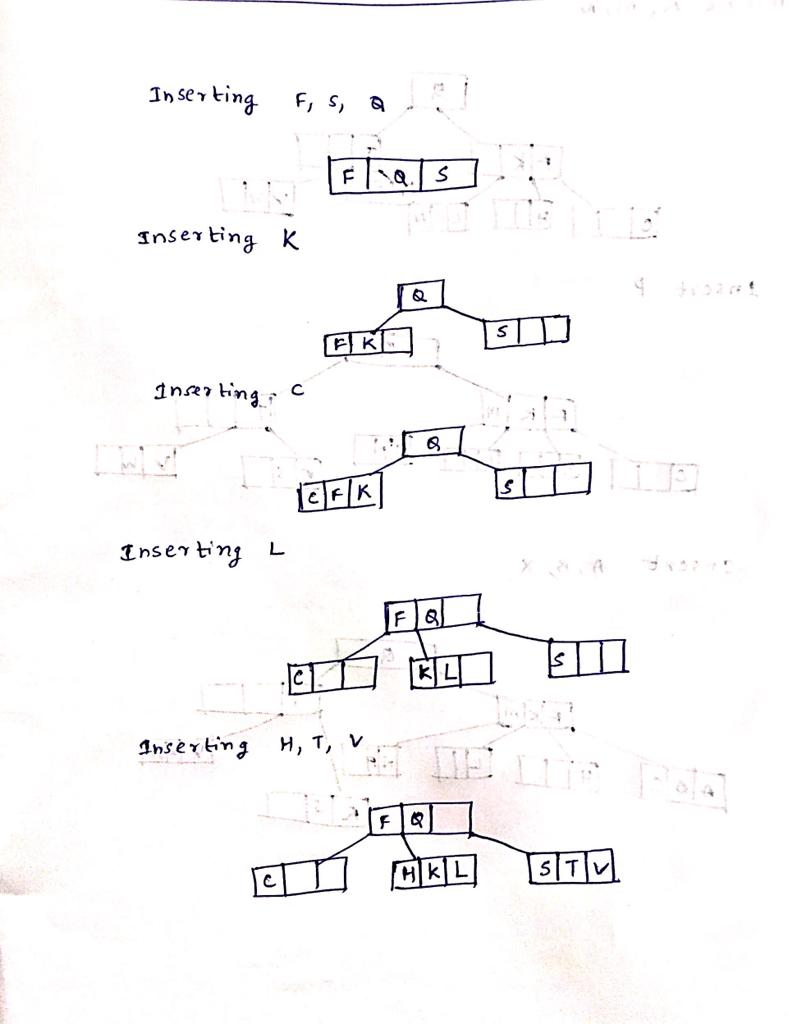
\includegraphics[scale=0.4]{WhatsApp Image 2020-04-06 at 3.14.35 AM.jpeg}
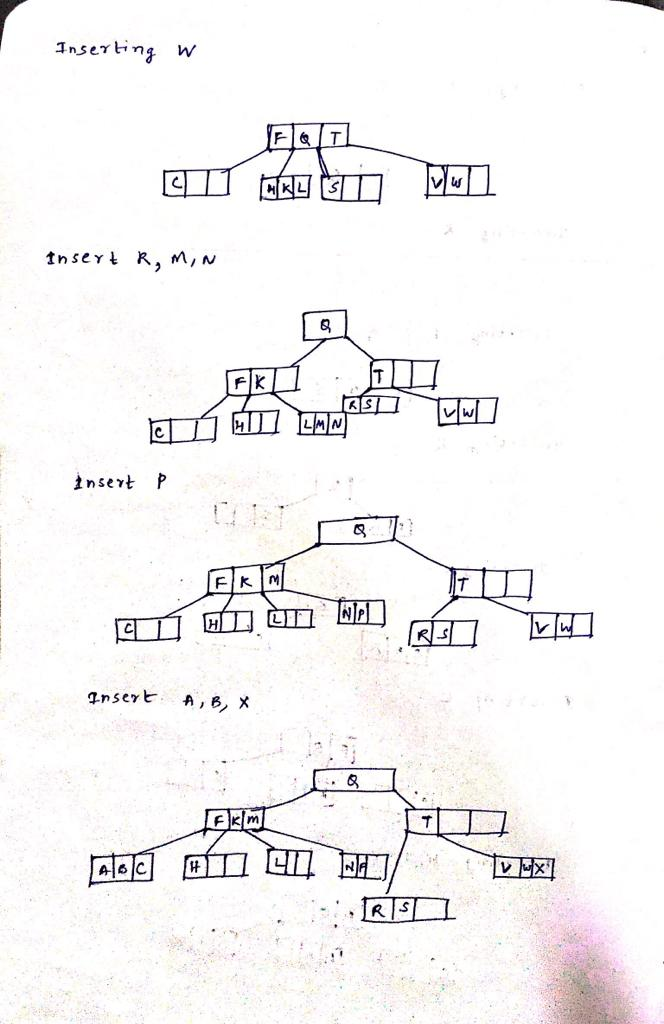
\includegraphics[scale = 0.4]{WhatsApp Image 2020-04-06 at 3.14.48 AM.jpeg}
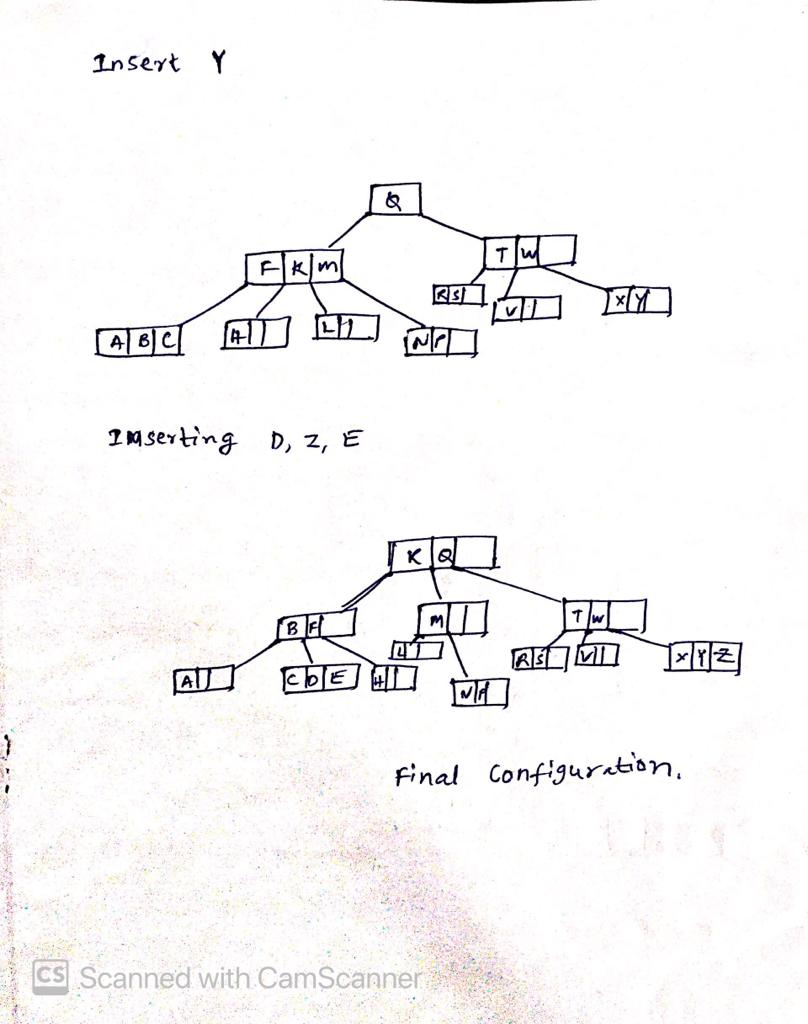
\includegraphics[scale = 0.4]{WhatsApp Image 2020-04-06 at 3.15.02 AM.jpeg}


\end{document}

